\documentclass[a4paper,12pt]{article}
\usepackage[latin1]{inputenc}
\usepackage[spanish]{babel}
\usepackage[dvips]{epsfig}
\usepackage{amsmath}
\usepackage{color}
\usepackage{graphicx}
\setlength{\textheight}{235mm}
\setlength{\textwidth}{168mm}
\setlength{\oddsidemargin}{0pt}
\pagestyle{empty}

\begin{document}
\mbox{}\vspace*{-45mm}

{\centering
{\small\sc Escuela T�cnica Superior de Ingenieros de Caminos, Canales y
Puertos (Madrid)}\\*[4mm]
{\Large\bf M�todo de los Elementos Finitos (2022-2023)}\\*[4mm]
PR�CTICA 8: Tecnolog�a de elementos \\*[4mm]
}

Sobre la c�pula esf�rica abierta de la figura act�an las cargas puntuales que
se indican en dicha figura.

Este es un ejemplo cl�sico
para analizar el comportamiento de elementos l�mina, que en este ejercicio
se resolver� utilizando elementos s�lidos tridimensionales. La geometr�a
del problema, las condiciones de contorno y las cargas aplicadas se muestran en la figura, teniendo el 
radio, el espesor y las propiedades del material los siguientes valores:
\begin{align}
R&=10 \\
t&=0.04 \\
E&=6.825 \cdot 10^7 \\
\nu&=0.3
\end{align}

El objetivo es discutir los resultados obtenidos con mallas de $10 \times 10$ y 
$50 \times 50$ elementos (con un s�lo elemento en el espesor), con formulaciones
de elementos isoparam�trica, mixta y de deformaciones supuestas;
comparando el valor del desplazamiento radial del punto $A$ con el valor de
referencia\footnote{Sim�, J.C., Fox, D.D. and Rifai, M.S. {\em On a stress
resultant geometrically exact shell model. Part II: The linear theory:
Computational aspects}. Computer Methods in Applied Mechanics and Engineering,
Vol 73, pp 53--92, 1989}
$u_A=0.093$.

\begin{center}
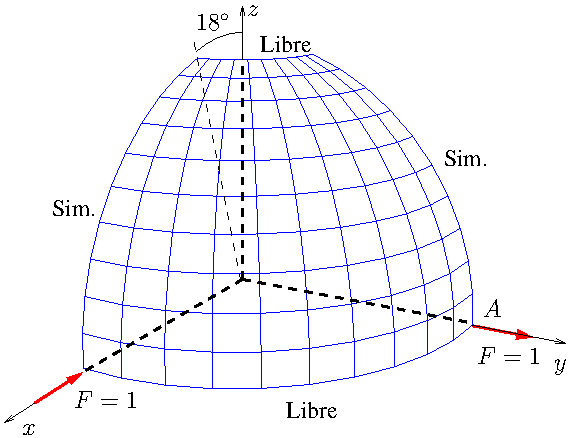
\includegraphics[width=0.6\textwidth]{esfera}
\end{center}
%\noindent
\end{document}
